\documentclass{article}
\usepackage[T1]{fontenc}
\usepackage{graphicx,booktabs,amsmath,amssymb}
\usepackage{hyperref}
\usepackage[preprint]{icml2026}
\urlstyle{same}
\hypersetup{pdfsubject={Research preprint on EEG window classification}}
\icmltitlerunning{Regional Evidence and Bilateral Interactions for EEG Classification}
\makeatletter\let\inputrows\@@input\makeatother
\newcommand{\tm}{T-MoE}
\newcommand{\logit}{\operatorname{logit}}
\begin{document}
\twocolumn[
\icmltitle{Regional Evidence and Bilateral Interactions\\
for EEG Window Classification}
\begin{icmlauthorlist}
\icmlauthor{Anonymous authors}{draft}
\end{icmlauthorlist}
\icmlaffiliation{draft}{Affiliation withheld in this preprint}
\icmlcorrespondingauthor{Project repository}{github.com/xiaobri/T-MOE/issues}
\icmlkeywords{electroencephalography, mixture of experts, partial information decomposition, paired ranking}
\vskip 0.3in
]
\printAffiliationsAndNotice{}
\begin{abstract}
Reflecting a scalp EEG swaps the two hemispheres without changing the recorded window. We ask which evidence a mixture of experts should average across this transformation and which it should retain in the recorded orientation. Our classifier, \tm{}, pools regional and matched positive--negative scores across orientations, preserves electrode order for spatial and spectral features, and uses a partial information decomposition (PID) to score interactions between native and reflected expert decisions. On 166,079 validation windows with 2.09\% positives, mean positive-class F1 across two seeds rises from 69.7870\% for the six-expert baseline and 72.0318\% for its refreshed-pair extension to 73.0240\%. Giving the baseline the same four views and head history yields 69.9280\%. The largest mean reductions occur when removing regional fusion (0.7653 F1 points) or matched ranking (0.5174). Removing bilateral PID costs 0.0921 points. The validation split guided development. Selecting checkpoints and thresholds on other inferred subjects gives 72.6689\%, which limits how precisely the primary result can be interpreted.
\end{abstract}

\section{Introduction}
A four-second EEG window can contain a brief, lateralized transient and a slow deflection shared across the scalp. Left--right reflection preserves the timing of both, while exchanging the side on which the transient appears. Removing a fitted slow trend changes the prominence of both. A classifier that averages every feature across these transformations makes the same invariance assumption for a regional expert's confidence and for the spatial distribution of scalp power. We test a weaker assumption: pool estimates of regional evidence, and let the spatial and spectral readouts retain their electrode ordering.

We study this question in a six-expert detector with five frozen regional sources and a trainable global expert. A previous study improved this detector by pooling time segments and comparing positives with previously sampled negatives from similar acquisitions \citep{predecessor}. That predecessor already achieved 72.0318\% mean F1. It provides a more informative reference for the new design than a comparison to the original detector alone. We adapt the pair-based readout to EEG-derived backgrounds and measure whether the joint responses of an expert to a window and its reflection add information beyond the marginal responses.

Our evaluation addresses two questions. First, how much of the gain survives when the baseline receives the same input views and access to earlier classifier heads from its own training run? Second, when the final classifier scores a window, which terms change the positive decision? For the latter we retain the trained weights and recompute operating points after removing each contribution. We also report how these effects change when the threshold and epoch must transfer to a held-out group. Both questions concern binary window labels in the source corpus. Clinical event detection over a continuous recording would require event annotations and a different evaluation unit.


\begin{figure*}[t]
\centering
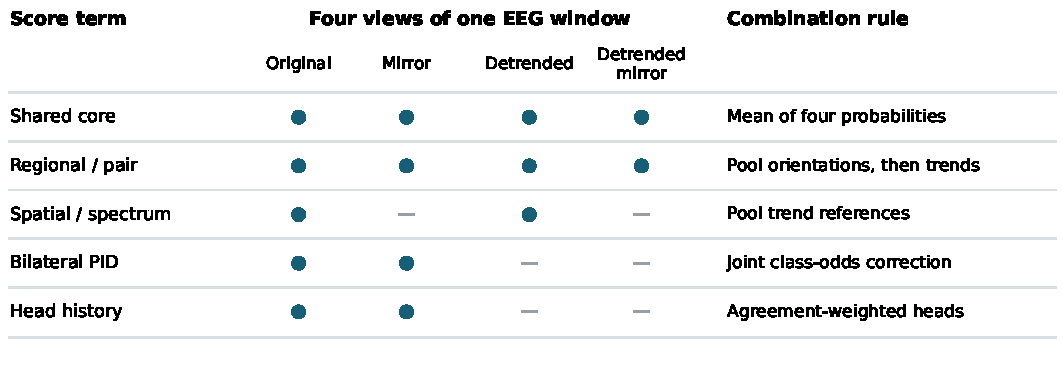
\includegraphics[width=0.96\textwidth]{figures/view-routing.pdf}
\caption{How one EEG window reaches the classifier. Each column is one transformation of that window. The marks show which scores enter each part of the final decision. Regional and matched scores pool mirror pairs. The two scalp readouts retain electrode orientation. The last two rows compare native and mirrored scores and operate on the original trend reference.}\label{fig:architecture}
\end{figure*}

\section{Method}
\subsection{Shared experts and window-level evidence}
Figure~\ref{fig:architecture} shows which branches consume each view. The input $x\in\mathbb{R}^{19\times2000}$ comprises four seconds at 500 Hz. Five frozen EfficientNetV2-S-family sources \citep{tan2021,predecessor} supply frontal, left-temporal, right-temporal, centro-parietal and occipital expert representations. Each receives all 19 input channels. A two-layer Transformer fuses the five 128-dimensional representations into a sixth expert. A dense router with softmax temperature 2 mixes the six pairs of logits. We write $c(x)$ for the positive-minus-negative margin of the baseline. A regional source name denotes how its weights were obtained and does not establish where a waveform originated in the brain.

The extended model adds four successive \emph{margin increments}. The regional increment $r$ collects the learned refinements to the shared core, including peak-shape features and learned pooling over eight time blocks per source. The matching increment $m$ adjusts the resulting margin using regional feature differences between positives and previously observed negatives. The training procedure fits 32 background groups on waveform descriptors. Soft membership weights guide the selection of up to 16 earlier controls from a 2,048-entry history. This compares the positive to a range of risks within similar backgrounds. Only fitted coefficients are needed for the pair-based readout at inference.

The spatial increment $s$ measures how band-limited activity at an electrode differs from its spatial context. It summarizes both standardized traces and conditional innovations relative to other electrodes. The final increment $v$ comes from a time-resolved spectrum: it maps 12 frequency bands and 32 time bins to a $5\times5$ scalp grid and fits a small convolutional encoder. \citet{wang2026} motivate this representation through EEG spectrum videos. Here the encoder trains from scratch using the same window labels as the detector. The stages act in sequence, so an increment denotes the change from its immediate input score. This distinction matters when a later stage uses an earlier score as a feature.

\subsection{A different pooling rule for each type of evidence}
Let $M$ exchange eight homologous electrode pairs and fix three midline leads. Let $D$ remove each channel's least-squares quadratic trend over the window. We evaluate $x$, $Mx$, $Dx$ and $MDx$. In the following, $u\in\{0,1\}$ indexes the native or detrended input, and $b\in\{0,1\}$ the original or reflected orientation. For a given trend choice define
\begin{align}
a_u &= \tfrac12\sum_{b=0}^{1}(r_{ub}+m_{ub}),\\
g_u &= a_u+s_{u0}+v_{u0}.
\end{align}
Thus a regional or pair increment contributes in both orientations, while a spatial or spectrum increment retains the recorded orientation for each trend choice.

We weight the two trend choices using a measure of how consistently the slow deflection appears across channels. We compute the empirical percentile $q(x)$ of that measure against the first 4,096 scheduled training windows, and set $w(x)=0.25+0.5q(x)$. A higher percentile gives more weight to the detrended view. The pooled contribution is
\begin{equation}
G(x)=(1-w(x))g_0+w(x)g_1. \label{eq:stage}
\end{equation}
The restricted weight range retains evidence from both references even at the extremes of the training distribution.

\subsection{Bilateral interaction and the final decision}
For each of five regional scores and the core score, let $(A,B)$ be its values on the native window and its reflection. We quantize each coordinate into five levels with shared training-derived boundaries. Class-conditional joint counts are symmetrized in $(A,B)$. This defines a two-source prediction problem with the binary label as target. The sources are responses to transformations of one observation. Their dependence does not imply two independently measured physiological processes.

Following the fixed-marginal coupling formulation of \citet{bert2014}, we estimate how the observed joint class evidence differs from that of a coupling preserving the separate source--label marginals. The model converts this difference into six bounded local log-odds features, one per score pair. A regularized positive--negative fit on prior training comparisons maps the features to an additive correction $J(x)$. Appendix~\ref{app:implementation} gives the estimator and its smoothing. The final correction is a predictive feature in log-odds units. The change in F1 after removing it is an empirical effect, not an information quantity.

Let $\sigma$ denote the sigmoid and $c_{ub}$ the current core margins. We average the four \emph{probabilities} and convert back to a margin. We also score the current native and reflected features with earlier heads from the same seed, weighting earlier epochs by recency and agreement between orientations. Let $H(x)$ be their weighted native margin, including the current head, minus the current native margin. The deployed score is
\begin{align}
C(x)&=\logit\!\left(\tfrac14\sum_{u,b}\sigma(c_{ub})\right),\\
p(x)&=\sigma\big(C(x)+H(x)+G(x)+J(x)\big). \label{eq:full}
\end{align}
Every term can be computed for one EEG window. The historical heads reuse current-window encoder features. Inference uses each seed separately and requires four passes through each frozen source.

\section{Evaluation}
\paragraph{Data and selection.}
The original Xiehe manifest assigns 731,610 windows to training (190,413 positive) and 166,079 to validation (3,471 positive). The endpoint is the manifest's positive binary window label. The supplied metadata do not establish an adjudicated diagnosis for that label. We retain the original split and channel order. For each seed in $\{3,42\}$ we evaluate every checkpoint from 20 epochs at the 99 thresholds from 0.01 to 0.99. We select on positive-class F1, $2TP/(2TP+FP+FN)$, and average the two selected seed scores. All primary results use predictions replayed from raw EEG. Appendix~\ref{app:protocol} documents sampling, tie handling and replay checks.

\paragraph{Controls.}
All four primary methods share the five source checkpoints, input length, sampled rows and batch order per seed, learning rate, batch size and number of AdamW updates. The second baseline also shares the four views and same-seed history rule in Eq.~\eqref{eq:full}. The refreshed-pair predecessor uses its published native-input protocol. The full method has 2,839,680 trainable parameters versus 365,576 for the original baseline, and adds auxiliary supervision from previously sampled windows. Matching training draws and updates therefore leaves differences in capacity and computation. Appendix~\ref{app:training} reports separately trained controls at the larger parameter count.

\begin{table}[t]
\caption{Positive-class validation F1 (\%). Each seed uses its own selected epoch and threshold.}\label{tab:primary}
\centering\small
\begin{tabular}{@{}lrrr@{}}
\toprule Model & Seed 3 & Seed 42 & Mean\\ \midrule
\inputrows tables/primary.tex
\bottomrule
\end{tabular}
\end{table}

\section{Results}
As Table~\ref{tab:primary} shows, \tm{} improves mean F1 by 3.2369 points over the native baseline, 3.0960 over its view- and history-matched counterpart, and 0.9922 over the refreshed-pair predecessor. At its selected threshold, seed 3 finds 2,515 positives with 920 false positives and 956 misses. Seed 42 finds 2,550 with 945 false positives and 921 misses. The paired 95\% recording-folder bootstrap intervals for the three gains are $[1.50,5.65]$, $[1.27,5.66]$ and $[0.18,1.84]$ points, respectively. These intervals condition on the selected models and operating points.

\begin{figure*}[t]
\centering
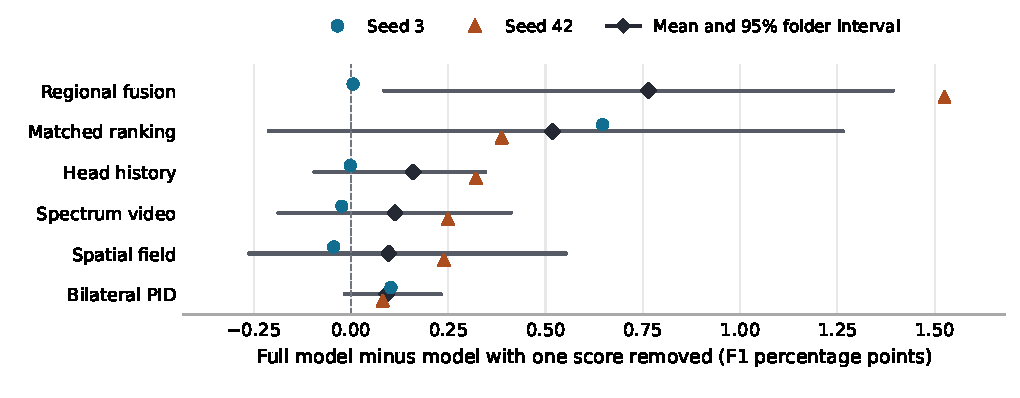
\includegraphics[width=0.88\textwidth]{figures/paired-ablation.pdf}
\caption{Which score terms contribute to the final decision? Each marker compares the full and ablated readouts after each has selected its own epoch and threshold. Positive values favor the full model. Lines are paired 95\% recording-folder bootstrap intervals for the two-seed mean at the selected operating points.}\label{fig:effects}
\end{figure*}

\paragraph{Regional and pair evidence account for the largest mean gains.}
On the final training trajectory, the shared core with four views and head history scores 69.9119\%. Adding the pooled regional increment gives 72.1933\%, and adding matched ranking brings the mean to 72.6990\%. In the reverse experiment, deleting regional fusion from the complete readout costs 0.7653 points. Most of this difference comes from seed 42. Deleting matched ranking costs 0.5174 points and lowers both seeds (Figure~\ref{fig:effects}). These estimates answer different questions because later stages depend on earlier scores and can move the best operating point. Neither series partitions the entire gain into independent effects.

\paragraph{Bilateral PID has a smaller effect.}
Deleting $J(x)$ gives 72.9319\% with operating points reselected, a decrease of 0.0921 points. Both seeds decrease, but the conditional folder interval for this gain spans zero ($[-0.016,0.231]$). At the original operating points, removing the same term gives 72.7877\%. Weighting the two trend choices equally instead of by coherence gives 73.0046\%. These results put the incremental value of each design choice in scale: the equal-weight model already exceeds 73\% on this validation split.

\paragraph{Transfer across inferred subjects.}
We held out each of 71 subject names inferred from validation directories, selected the epoch and threshold on the remaining names, and pooled the held-out confusion counts. The full model gives 72.6689\%, compared with 71.6114\% for the predecessor. Deleting the spectrum-video score gives 72.7716\% under this rule, reversing the ordering seen under full-validation selection. Three inferred names occur in both training and validation. Removing their windows at the original operating points yields 71.0716\% for \tm{} and 70.2115\% for the predecessor. The names are proxies for identity. Neither analysis supplies an independent clinical test.

\section{Related Work}
Interaction-aware mixtures model how sources jointly influence a prediction \citep{xin2025}. Sample-level multimodal interaction estimators \citep{yang2025} and decision-level PID analyses \citep{fang2026} motivate measuring what changes when two sources are considered jointly. Our exchange-symmetric variables are paired EEG views, and our readout uses a finite-alphabet coupling contrast. The sample-wise estimator of \citet{yang2025} and the language-conditioned estimator of \citet{fang2026} address different estimation problems.

Cross-batch memory supplies comparisons beyond a single mini-batch \citep{wang2020}. Our predecessor adapts this idea to previously observed negative EEG windows \citep{predecessor}. In \tm{}, waveform-derived background memberships guide those comparisons. The auxiliary objective also draws on cost-sensitive metric optimization \citep{mao2025} and class-conditional distribution balancing \citep{zhao2026}. We use these ideas within a detector trained on a fixed stream of windows. The threshold policy and the score terms can therefore be evaluated independently of changes to the sampling schedule.

\section{Discussion}
The clearest evidence is for retaining regional information over time and comparing similar-background windows. Explicit bilateral interaction contributes a smaller, repeatable change in direction across two seeds. Its magnitude is sensitive to the operating point, and recording-level uncertainty includes zero. Retaining electrode orientation or suppressing drift may suit this corpus differently from another montage or acquisition protocol.

Method development repeatedly used the same validation split. The experiment archive contains 559 completed two-seed run directories spanning 558 method names, including earlier development work. Such repeated selection can favor promising fluctuations \citep{cawley2010}. Applying the chosen fusion rule to corresponding checkpoints of an earlier training repeat gives 72.9715\%. Together with the group-transfer and overlap analyses, this limits the precision of the 73.0240\% estimate. Appendix~\ref{app:external} tests the source-locked classifiers in four external hospitals, and Appendix~\ref{app:activation} measures how their six core expert responses vary across sites. Verified patient identities and clinically adjudicated endpoints would allow a patient-level assessment.

\section*{Impact Statement}
A more sensitive EEG window classifier could help prioritize segments for expert review, but false positives also increase review burden. Here the unit is a four-second window, and the labels, patient identities and operating points have not been validated for clinical deployment. The aggregate results permit scrutiny of error counts and model selection without distributing individual recordings.

\bibliography{references}
\bibliographystyle{icml2026}
\clearpage
\appendix
\onecolumn
\section{Experimental protocol and implementation}\label{app:protocol}
\paragraph{Data and input.}
The training split contains 541,197 negative and 190,413 positive windows. The corresponding validation counts are 162,608 and 3,471. The loader selects channels 1--19 in their stored order, divides the stored amplitude by $10^{-3}$, and takes the first 2,000 samples per channel with right zero-padding for shorter inputs. No ECG or EMG input is constructed. The split audit found no exact file path shared across training and validation. It did find three shared parent-directory names. Their interpretation is discussed in Appendix~\ref{app:robust}. We use the manifest label as supplied and make no assumptions about unavailable annotation or adjudication details.

\paragraph{Optimization and selection.}
For each seed, every epoch uses 19,355 negative and 645 positive draws. The sampler draws without replacement within the epoch. The batch size is 128, giving 156 full batches and one batch of 32. Over 20 epochs this gives 400,000 sampled positions and 3,140 AdamW updates. Learning rate is $5\times10^{-4}$, weight decay 0.01, focal-loss $\alpha=0.85$, and $\gamma=2$. Training uses FP32. Fusion width is 128 with two layers, four attention heads and dropout 0.3. Router width is 128 with two layers and dropout 0.5. All methods use the historical threshold grid. For a tied maximum within an epoch we select the lowest threshold. Across tied epochs we select the latest epoch. A positive decision requires $p>t$. Neither class predictions nor probabilities are averaged across seeds.

The shared core receives its original loss gradients. The extension fits its regional and spatial heads, auxiliary ranking and classification terms on the scheduled windows. The spectrum head also receives an auxiliary loss with false-positive and false-negative costs derived from earlier training confusion estimates, evaluated across background groups. The training code caps extreme background weighting and fits the auxiliary comparison statistics using the labels of earlier sampled windows. The number of optimizer updates therefore understates the additional supervision and arithmetic. The two-seed baseline with the same four views and histories controls specifically for inference access. It retains the smaller trainable parameter count.

\paragraph{Raw-input verification.}
We scored all validation windows three ways at the selected operating points: the exported single-seed detector, an implementation that expands its branch outputs, and a replay that recomputes each view and head from raw EEG. Across these implementations the 166,079 threshold decisions agree for each seed. Small continuous-score differences occur in some windows near PID bin boundaries. Removing the measured PID offset from raw predictions at the released thresholds also reproduces the ablation's confusion counts. The shared core's cached predictions agreed with the cached baseline trajectory at all 20 epochs for both seeds. Raw-trained and cached-trained baseline trajectories have slightly different selected scores, so each table identifies the reference it uses.

\subsection{Drift, interaction and history estimators}\label{app:implementation}
For the drift statistic, average each channel over 50 consecutive blocks of 40 samples and subtract its temporal mean. Project each resulting vector onto the orthonormal linear and quadratic components and divide by its temporal Euclidean norm (floored at $10^{-6}$). Let $d_i\in\mathbb R^2$ denote the two coefficients for channel $i$. The coherence score is
\begin{equation}
k(x)=\frac{\|\frac{1}{19}\sum_i d_i\|_2^2}{0.02+\frac{1}{19}\sum_i\|d_i\|_2^2}.
\end{equation}
The percentile in Eq.~\eqref{eq:stage} is the fraction of the 4,096 training reference values at or below $k(x)$. This calculation uses no validation reference windows or labels.

For the bilateral estimator, each of the six coordinates uses the pooled orientation-specific training quintiles to define a $5\times5$ table. Counts for $(a,b)$ and $(b,a)$ receive equal weight. Each class table is smoothed by a product-of-marginals prior with mass 24 and a 0.05 pseudocount per cell. The model updates counts after scoring training batches. For each coordinate, let $P_y$ be the resulting class-conditional table. Under an equal class prior, the coupling step seeks the least informative joint $Q$ with the same $(Y,A)$ and $(Y,B)$ marginals:
\begin{equation}
\min_{Q:\,Q(Y,A)=P(Y,A),\;Q(Y,B)=P(Y,B)} I_Q(Y;A,B).
\end{equation}
The implementation uses up to 32 alternating updates and a feasibility repair when needed. Exchange symmetry makes the two single-source marginals identical. In that idealized problem the coupling $A=B$ attains the single-source lower bound. For the \emph{local predictive score} we use the numerical coupling, with a separate smoothing step to avoid unstable log odds in low-mass cells. Write $R_y=0.9Q_y+0.1P_y(A)P_y(B)$. The feature for the observed bin is
\begin{equation}
j(a,b)=\operatorname{clip}_{[-2,2]}\!\left(\log\frac{P_1(a,b)}{P_0(a,b)}
                         -\log\frac{R_1(a,b)}{R_0(a,b)}\right).
\end{equation}
A regularized logistic update on matched feature differences fits coefficients for the six-dimensional vector $j$. The correction is $J(x)=2.5\tanh((j-\bar j)^\top\beta/2)$. Its center and coefficients are estimated on training draws. No other validation window or group identifier enters this prediction.

For the history term, let $c_{t,00}$ and $c_{t,01}$ be the current window's native and reflected margins under the head saved at epoch $t$. At selected epoch $e$ define
\begin{equation}
b_t=\frac{2^{(t-e)/4}}{1+(c_{t,00}-c_{t,01})^2},\qquad
H=\frac{\sum_{t=1}^{e} b_t c_{t,00}}{\sum_{t=1}^{e}b_t}-c_{e,00}.
\end{equation}
The four-epoch half-life favors recent heads. The denominator in $b_t$ additionally reduces the weight of heads whose score for this window changes strongly under reflection. Snapshots never extend beyond the checkpoint being evaluated.

\section{Readout ablations on the final training trajectory}\label{app:ablate}
We saved the core margin and the four stage increments for every validation window, view, epoch and seed. To remove an increment, we zero only its direct contribution to Eq.~\eqref{eq:full}. Later stages still see the representations and intermediate margins on which they were trained. These experiments estimate dependence of the deployed decision on each score term. A model trained from initialization without the branch could adapt its other weights and give a different answer.

\begin{table}[ht]
\caption{Single-term deletion on the original validation set. Except in the final column, each arm reselects its epoch and threshold separately for each seed. Loss is the full-model mean minus the arm mean in percentage points. Locked mean holds the full model's epoch \emph{and} threshold fixed for each seed. All F1 columns are in percent.}\label{tab:drop}
\centering\small
\begin{tabular}{@{}lrrrrr@{}}
\toprule Term removed & Seed 3 & Seed 42 & Mean & Loss (pp) & Locked mean \\ \midrule
\inputrows tables/drop.tex
\bottomrule
\end{tabular}
\end{table}

\begin{table}[ht]
\caption{Operating points for Table~\ref{tab:drop} after reselection. Each column group refers to all 166,079 windows. The threshold $t$ is applied with a strict inequality.}\label{tab:ops}
\centering\small
\begin{tabular}{@{}lrrrrrrrrrr@{}}
\toprule & \multicolumn{5}{c}{Seed 3} & \multicolumn{5}{c}{Seed 42} \\
\cmidrule(lr){2-6}\cmidrule(l){7-11}
Term removed & Epoch & $t$ & TP & FP & FN & Epoch & $t$ & TP & FP & FN \\ \midrule
\inputrows tables/operating.tex
\bottomrule
\end{tabular}
\end{table}

The regional increment changes the scale of the final margin. Removing it while retaining thresholds 0.91 and 0.87 reduces mean F1 to 28.5753\%. Once the ablated scores select their own thresholds (0.58 and 0.57), mean F1 recovers to 72.2586\%. A locked-threshold ablation therefore confounds a change in score scale with a change in separability. Reselection also changes the ranking epoch, as the pair-deletion row in Table~\ref{tab:ops} illustrates. By comparison, deleting PID leaves the selected epochs unchanged. Under reselection the PID term adds one true positive and removes eight false positives for seed 3, while adding 16 true positives and 20 false positives for seed 42.

\begin{table}[ht]
\caption{Cumulative reconstruction from the same checkpoints. Each row optimizes its own operating point. The order follows the model's dependency chain. The shared core in this table is the core of the cached training trajectory.}\label{tab:chain}
\centering\small
\begin{tabular}{@{}lrrrr@{}}
\toprule Included evidence & Seed 3 & Seed 42 & Mean F1 (\%) & Step (pp)\\ \midrule
\inputrows tables/chain.tex
\bottomrule
\end{tabular}
\end{table}

The cumulative reconstruction (Table~\ref{tab:chain}) gives a second way to read the same scores. The spatial increment slightly reduces mean F1 when appended directly after ranking, yet removing it from the complete detector reduces F1. The spectrum increment then adds 0.2679 points after the field is present. Sequential gains depend on which later scores are available, so summing single-deletion losses would give a misleading attribution.

\section{View policy and training controls}\label{app:training}
\begin{table}[ht]
\caption{View policy on identical checkpoints. Only the pooling of the stage increments changes. Core pooling, history, PID, the threshold grid and the seed-specific selection procedure are held fixed. F1 is in percent.}\label{tab:views}
\centering\small
\begin{tabular}{@{}lrrr@{}}
\toprule Stage pooling policy & Seed 3 & Seed 42 & Mean \\ \midrule
\inputrows tables/views.tex
\bottomrule
\end{tabular}
\end{table}
The native-only row applies the stage increments measured on the unreflected, original window. In the next two rows only the named increments are averaged, and all other increments keep their native values. Averaging all four increments over all four views gives 72.9167\%. Preserving the recorded orientation for spatial and spectrum features with equal trend weights raises the mean to 73.0046\%. Coherence weighting adds a further 0.0194 points. The absolute differences between the last four policies are small compared with the gain above the original single-view baseline.

\begin{table}[ht]
\caption{Separately trained controls on the original validation set, evaluated on raw input. Each row has its own training trajectories and selected checkpoints. The first row uses the cached-execution baseline. The five larger arms share parameter count and training schedule.}\label{tab:controls}
\centering\small
\begin{tabular}{@{}lrrrr@{}}
\toprule Training condition & Trainable parameters & Seed 3 & Seed 42 & Mean F1 (\%)\\ \midrule
\inputrows tables/training.tex
\bottomrule
\end{tabular}
\end{table}
The single-group control retains the extended neural architecture but supplies one anonymous background group. Online spectral grouping estimates 24 groups from the incoming spectral representation. The stationary arm fits 32 groups using descriptors of two halves of each training window. Soft matching then uses uncertain membership to weight previous negatives. A further neighboring-group control changes support for sparse groups. Across these equal-size runs, soft matching reaches 72.3240\%, compared with 70.9315\% under a single group. This comparison concerns the training treatment of backgrounds in those earlier variants. It does not isolate a training-time deletion of the final PID head. The controls also do not equate end-to-end inference FLOPs with the original baseline.

\section{Uncertainty and grouping sensitivity}\label{app:robust}
We used two kinds of groups because they address different sources of variation. For the \textbf{paired bootstrap}, we sampled 72 full validation recording folders with replacement 3,000 times. For each resample we used identical multiplicities across seeds and methods, recomputed each seed's F1 from summed TP/FP/FN, and averaged the two score differences. Table~\ref{tab:held} reports the 2.5th and 97.5th percentiles. The checkpoints and thresholds had already been selected on the complete validation split. These intervals describe variation across folders at those settings. Training variability and repeated method selection are outside their scope.

For \textbf{group-held selection}, we instead grouped windows by the inferred subject name in their parent directory. For each of the 71 names and each arm, we selected an epoch and threshold using the remaining 70 names and applied them once to the held-out name. We summed counts across the 71 held-out groups before computing F1 for each seed. This gives each window the same weight when pooling counts. It assesses transfer of the operating point within the source validation corpus. No training weights were refit within these folds.

\begin{table}[ht]
\caption{Operating-point transfer and uncertainty of individual ablations. The first three columns are group-held F1 (\%). The last column is a separate analysis on the original full-validation operating points and reports the paired folder interval for deleting the named term, in points (full minus ablated).}\label{tab:held}
\centering\small
\begin{tabular}{@{}lrrrr@{}}
\toprule Term removed & Held seed 3 & Held seed 42 & Held mean & Original gain, 95\% interval\\ \midrule
\inputrows tables/held.tex
\bottomrule
\end{tabular}
\end{table}

\begin{table}[ht]
\caption{Mean F1 (\%) by evaluation policy. Exclusion removes 2,582 windows, including 394 positives, from the three suspected shared names and retains the original operating points. The reduced evaluation has 163,497 windows and 3,077 positives.}\label{tab:sensitivity}
\centering\small
\begin{tabular}{@{}lrrr@{}}
\toprule Model & Original & Group-held selection & Suspected overlap excluded\\ \midrule
\inputrows tables/sensitivity.tex
\bottomrule
\end{tabular}
\end{table}

Only the regional deletion has a conditional folder interval wholly above zero in Table~\ref{tab:held}. Pair deletion lowers both primary seed scores, while its interval is wide enough to include zero. Removing spectrum video improves the held mean by 0.1027 points despite lowering the primary mean. Table~\ref{tab:sensitivity} also shows that removing the suspected overlapping names decreases absolute F1 for every method. Both findings argue for reporting the method's advantage relative to controls alongside the uncertainty in its absolute score.

\clearpage
\section{Four-hospital evaluation with source-locked operating points}\label{app:external}

We applied the exported Xiehe classifiers to all 698,502 labeled windows from four external hospitals. Seed 3 used epoch 3 and threshold 0.91; seed 42 used epoch 9 and threshold 0.87. We retained the source preprocessing, PID tables and drift references. No target-site data were used to fit or select weights, epochs or thresholds.

The native baseline uses source epochs 2 and 5 (thresholds 0.81 and 0.82). The four-view, history-matched baseline uses epochs 13 and 8 (0.81 and 0.83). The refreshed-pair predecessor uses epochs 5 and 4 (both 0.95). We recomputed both baselines and matched the historical raw-input predictions to the same manifests, row order, labels and locked checkpoints \citep{predecessor}. All decisions use $p>t$.

\begin{table}[ht]
\caption{External positive-class F1 (\%). Each cell averages seed-specific F1. The final rows weight hospitals equally or pool their confusion counts within seed. Gain and its paired 95\% folder interval are in points versus the predecessor.}\label{tab:external-overview}
\centering\small
\begin{tabular}{@{}lrrrrrrr@{}}
\toprule Site & Windows (positive) & Baseline & Matched & Predecessor & T-MoE & Gain & 95\% interval\\ \midrule
\inputrows tables/external_overview.tex
\bottomrule
\end{tabular}
\end{table}

\begin{table}[ht]
\caption{T-MoE at its source-selected thresholds. Precision, recall, F1, average precision (AP) and AUROC are percentages.}\label{tab:external-operating}
\centering\small
\begin{tabular}{@{}lrrrrrrrrrr@{}}
\toprule Site & Seed & TP & FP & FN & TN & Precision & Recall & F1 & AP & AUROC\\ \midrule
\inputrows tables/external_operating.tex
\bottomrule
\end{tabular}
\end{table}

We resampled recording folders 5,000 times within each hospital, using the same draws across models and seeds. Qilu, Tiantan, Chifeng and Xi'an contribute 75, 99, 32 and 20 folders, respectively; 48, 44, 8 and 10 contain positive windows. These intervals condition on the four observed hospitals and the selected models. Folder names have no verified patient linkage.

\paragraph{Transfer at fixed thresholds.}
T-MoE exceeds the native baseline at three hospitals and falls by 1.72 points at Tiantan. Its equal-site gain is 2.66 points versus the native baseline ($[0.57,5.17]$) and 2.67 versus the matched baseline ($[0.62,5.21]$). It exceeds the predecessor at Qilu and Xi'an but gives up 0.30 points on the four-site mean ($[-1.08,0.81]$). Thus its 0.99-point source advantage over the predecessor does not transfer to the equal-site mean. Tiantan has 74.96\% mean recall but 27.89\% precision. Xi'an has 64.76\% precision but only 21.03\% recall.

\paragraph{Replay sensitivity.}
The native baseline column uses the archived raw decisions. The fresh native replay differed on two of 1,397,004 window--seed decisions, one each at Qilu and Tiantan for seed 42. Both archived scores were within 0.00017 of threshold. Substituting fresh counts changes either site mean by less than 0.007 F1 points. Independent raw-waveform checks covered the first, last and all disputed native batches per site; the matched baseline agreed on every checked decision. T-MoE's shared-encoder evaluation exactly reproduced direct detector outputs on the first and last batches of every site partition.

\clearpage
\section{Activation of the six core experts}\label{app:activation}

All six experts run on every view. For each expert we instead measure the router's softmax weight $\pi_{jv}$ and the head's own positive score $p_{jv}=\sigma(\ell_{jv,1}-\ell_{jv,0})$. We average each quantity over the four views of a window, then over windows with the same hospital and true label. The displayed values average the two seed-specific summaries. The five frozen regional heads give identical standalone scores across the two seeds. Their routing weights and the trained global head can vary by seed.

\begin{figure}[ht]
\centering
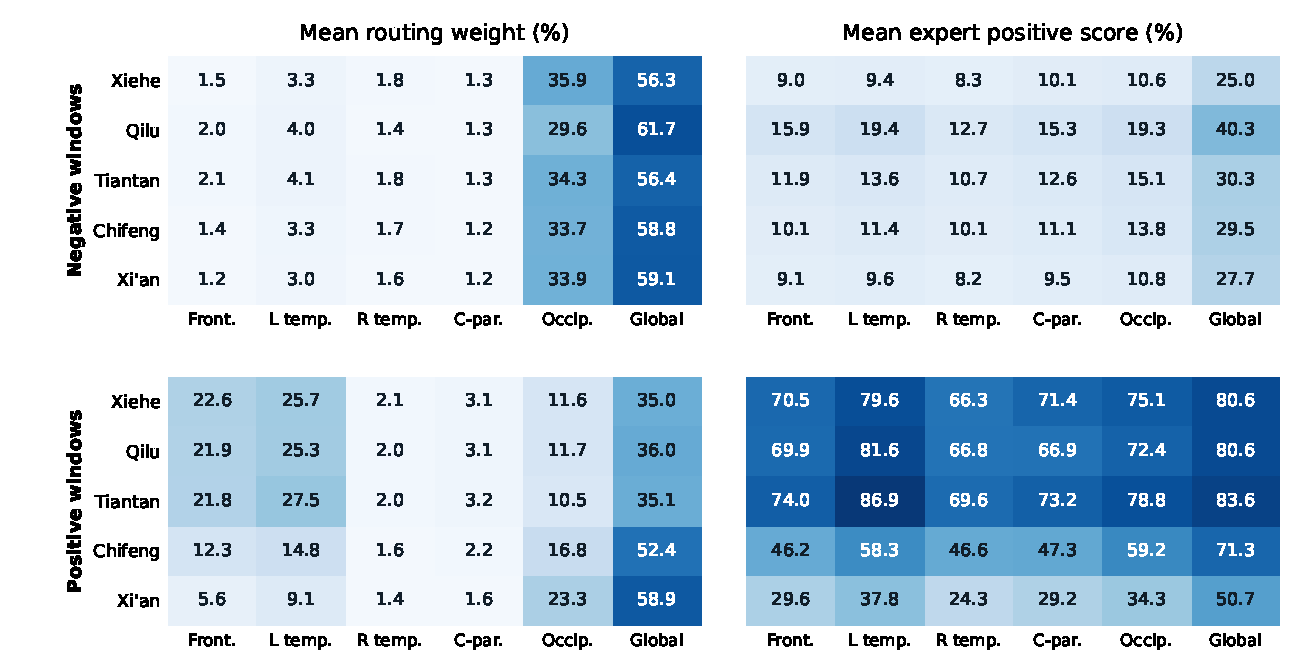
\includegraphics[width=0.94\textwidth]{figures/hospital-experts.pdf}
\caption{Activity by site and true label (\%). The left panels show routing mass, which sums to 100\% per row before rounding. The right panels show each head's positive score. Color scales are shared across label strata within each column.}\label{fig:hospital-experts}
\end{figure}

\begin{table}[ht]
\caption{Source validation activity (\%). Top share is the fraction of windows on which the expert receives the largest four-view mean routing weight.}\label{tab:expert-source}
\centering\small
\begin{tabular}{@{}lrrrrrr@{}}
\toprule & \multicolumn{2}{c}{Mean routing weight} & \multicolumn{2}{c}{Top share} & \multicolumn{2}{c}{Mean expert positive score}\\
\cmidrule(lr){2-3}\cmidrule(lr){4-5}\cmidrule(l){6-7}
Expert & Negative & Positive & Negative & Positive & Negative & Positive\\ \midrule
\inputrows tables/source_experts.tex
\bottomrule
\end{tabular}
\end{table}

On Xiehe negatives, the global and occipital experts receive 56.25\% and 35.90\% of routing mass. On positives the global share falls to 34.95\%, while left-temporal and frontal weights reach 25.68\% and 22.58\%. The right-temporal expert's own positive score rises from 8.27\% to 66.29\% despite receiving only about 2\% of the routing mass.

The global expert leads on negatives at all four external sites (56.41--61.68\%). On positives, Qilu and Tiantan assign about one quarter of the mass to the left-temporal expert. Xi'an assigns it 9.14\% and the global expert 58.93\%. The global expert's positive score on Xi'an positives averages 50.68\% versus 80.61\% on Xiehe. These shifts accompany lower Xi'an recall and do not establish which expert caused an error.

The aggregate file includes per-seed counts, routing-weight quartiles, native-view means and the mean signed weighted margin, $\frac14\sum_v\pi_{jv}(\ell_{jv,1}-\ell_{jv,0})$. Equation~\eqref{eq:full} also uses probability pooling, history and corrections. These summaries quantify core behavior; they do not identify the F1 effect of deleting an expert or localize a waveform to a brain region.

\end{document}
